\section{Properties of Limits}

\begin{recap}
  \begin{itemize}
    \item If $f(x)$ is arbitrarily close to $L$ whenever $x$ is sufficiently close to, \textit{but not equal to} $a$, then we say $\dlim_{x\to a}f(x) = L$.
    \item If the left-side limit and the right-side limit do not match up, we say that the (two-sided) limit does not exist.
    \item We can estimate limits numerically by evaluating $f$ at $x$-values close to (and on either side of) $a$.
    We look to see if the $y$-values are arbitrarily close to some real number.
    \item We can estimate limits graphically by visualizing the function values around $a$, and again trying to see if the $y$-values are arbitrarily close to some value.
  \end{itemize}
\end{recap}

We've estimated limits numerically and graphically, but these can be difficult without more tools at our disposal.
Here we'll build up some analytic methods of evaluating limits.
We'll start by building some general limit laws for any function.

\subsection*{Limit Laws In General}

We will now think about functions in general, and build some laws/properties to apply to limits, no matter the context.
These properties will all be based around some basic operations on functions: addition, multiplication, division, and some exponents.

\begin{imp}{Limit Laws and Properties}
  Let $f$ and $g$ be two functions, and assume that $\dlim_{x\to a} f(x)=L$ and $\dlim_{x\to a} g(x)=M$ for two real numbers $L$ and $M$. Essentially, assume both limits exist.
  Then:
  \begin{enumerate}
    \item $\dlim_{x\to a} [f(x)\pm g(x)] = \lim_{x\to a} f(x) \pm \lim_{x\to a} g(x) = L\pm M$
    \item $\dlim_{x\to a} cf(x) = c\lim_{x\to a} f(x)= cL$ for any constant multiple (coefficient) $c$.
    \item $\dlim_{x\to a} [f(x)\cdot g(x)] = \left[\lim_{x\to a} f(x)\right] \left[\lim_{x\to a} g(x)\right] = LM$
    \item $\dlim_{x\to a} \frac{f(x)}{g(x)} = \frac{\dlim_{x\to a} f(x)}{\dlim_{x\to a} g(x)} = \frac{L}{M}$ if $\dlim_{x\to a} g(x)\neq0$
    \item $\dlim_{x\to a} (f(x))^n = \left(\dlim_{x\to a} f(x) \right)^n = L^n$ for integers $n$. (If $n<0$, there's actually division going on: make sure you don't divide by 0.)
  \end{enumerate}
\end{imp}

\begin{note}{Explanations}\hspace{1cm}
  \begin{enumerate}
    \item Since the limit is concerned with what the $y$-value is arbitrarily close to, we can see that the operation is ``preserved" across the limit.
    Essentially, if one of the function values is arbitrarily close to something like 4, and the other is arbitrarily close to something lik 3, then the sum of the functions has to be close to 7.
    The following saying is helpful here: ``the limit of a sum (or difference) is the sum (or difference) of the limits.''
    \item Notice that a coefficient really represents repeated addition: $c\cdot f(x) = \underbrace{f(x) + f(x) + ...+ f(x)}_{c \text{ times}}$.
    \item ``The limit of a product is the product of the limits.''
    Limits preserve multiplication in the same way that they preserve sums.
    \item Dividing is really just multiplication by a reciprocal.
    The only thing we need to worry about is the same thing we always thing about: dividing by 0.\footnote{We'll investigate this more!}
    \item An exponent really represents repeated multiplication: $(f(x))^n = \underbrace{f(x) \cdot f(x) \cdot ... \cdot f(x)}_{n \text{ times}}$. We have to be careful with non-integer values of $n$. Like, for $f(x)^{1/2}$, our metaphor of repeated multiplication falls apart. \footnote{Again, we'll investigate this a bit more later.}
  \end{enumerate}
\end{note}

\subsection*{Examples}
Given $\dlim_{x\to 1} f(x) = 4$ and $\dlim_{x\to 1} g(x) = 2$, evaluate the following limits:
\begin{enumerate}
  \item $\dlim_{x\to 1}\left(\dfrac{f(x)-g(x)}{f(x)}\right)$

  When we consider $\dlim_{x\to 1}\left(\dfrac{f(x)-g(x)}{f(x)}\right)$, we should notice that the function $\dfrac{f(x)-g(x)}{f(x)}$ is really a combination of the two functions that we have information about.
  The operations are subtraction and division.
  We can use the properties above to re-write this limit:

  \begin{align*}
    \lim_{x\to 1}\left(\dfrac{f(x)-g(x)}{f(x)}\right) &= \frac{\dlim_{x\to 1} (f(x)-g(x))}{\dlim_{x\to 1} f(x)} & \text{Division Property (Property 4)}\\
    & = \frac{\left(\dlim_{x\to 1} f(x)\right)- \left(\dlim_{x\to 1} g(x)\right)}{\dlim_{x\to 1} f(x)} & \text{Difference Property (Property 1)}
  \end{align*}

  Now, we notice that we can input the values above, since we know that $\dlim_{x\to1} f(x) = 4$\footnote{Notice that since $\dlim_{x\to1}f(x)\neq0$, we're allowed to put this value in the denominator. Remember, we can't evaluate a limit using these properties if there's division by 0.} and $\dlim_{x\to 1}g(x) = 2$.

  \begin{align*}
    \frac{\left(\dlim_{x\to 1} f(x)\right)- \left(\dlim_{x\to 1} g(x)\right)}{\dlim_{x\to 1} f(x)} & = \frac{4-2}{4}\\
    &= \frac{2}{4} = \frac12
  \end{align*}

  So we can see that $\dlim_{x\to 1}\left(\dfrac{f(x)-g(x)}{f(x)}\right) = \frac{1}{2}$.

  \item $\dlim_{x\to 1} \left(3f(x)+\dfrac{2(g(x))^3}{5}\right)$

  Here, we have two functions added together, an exponent on one, and coefficients on each. We can again use the properties above.
  Again, we'll use the properties above:

  \begin{align*}
    \dlim_{x\to 1} \bigg( 3f(x) &\left.+\dfrac{2(g(x))^3}{5}\right) \\
    & = \left(\dlim_{x\to 1} 3f(x)\right) + \left(\dfrac{2(g(x))^3}{5}\right) & \text{Sum Property (Property 1)}\\
    &= 3\left(\dlim_{x\to 1} f(x)\right) + \dfrac{2}{5}\left(\dlim_{x\to1} (g(x))^3 \right) & \text{Coefficient Property (Property 2)}\\
    & = 3\left(\dlim_{x\to 1} f(x)\right) + \dfrac{2}{5}\left(\dlim_{x\to 1}g(x)\right)^3 & \text{Exponent Property (Property 5)}
  \end{align*}

  Again, we can input the values above, since $\dlim_{x\to1} f(x) = 4$ and $\dlim_{x\to 1}g(x) = 2$ are given.

  \begin{align*}
    3\left(\dlim_{x\to 1} f(x)\right) + \dfrac{2}{5}\left(\dlim_{x\to 1}g(x)\right)^3 & =3(4) + \dfrac{2}{5}(2)^3 \\
    &= 12 + \dfrac{2}{5}(8) = 12 + \dfrac{16}{5}\\
    & = \dfrac{76}{5}
  \end{align*}

  So the limit $\dlim_{x\to 1} \left(3f(x)+\dfrac{2(g(x))^3}{5}\right) = \dfrac{76}{5}$.
\end{enumerate}

We can see that these limit laws are very helpful for building our limit ``piece-by-piece.''
What happens, though, when we have some function or combination of functions that involves an operation or function type that is not covered in these properties?

One last thing to think about is a more generlized property for exponents.
Our property above only holds for integer exponents.

\begin{note}{Remember}
  Roots and radicals can be written as fraction exponents.
  \[\sqrt{x} = x^{1/2}\]
\end{note}

\subsection*{Square Roots}

Let's consider the function $y=\sqrt{x}$.
Specifically, we'll consider $\dlim_{x\to 0} \sqrt{x}$ first.

In the spirit of this chapter, we should start with numerical and graphical esimations.

\subsubsection*{Graphical Approximation}

Let's consider the graph of $y=\sqrt{x}$ around $x=0$.

\begin{figure}
  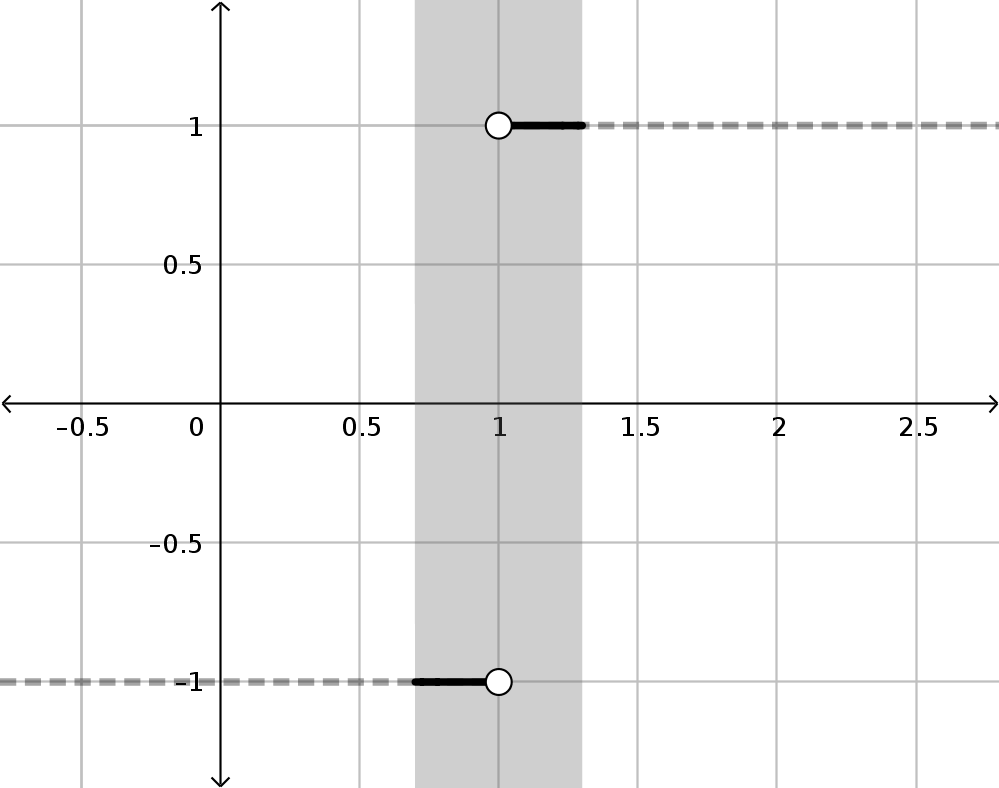
\includegraphics[scale=0.5]{./1_limits/images/1-2_graph3.png}
  \centering
\end{figure}

Consider this, and then we'll look at the numerical approximation, and summarize our findings after that.

\subsubsection*{Numerical Approximation}

\textbf{Left-Sided Limit}

\begin{tabular}{ccccc} \toprule
  $\bm{x}$ & $-0.5$ & $-0.1$ & $-0.01$ & $-0.001$ \\ \midrule
  $\bm{\sqrt{x}}$ & $\sqrt{-0.5}$ & $\sqrt{-0.1}$ & $\sqrt{-0.01}$ & $\sqrt{-0.001}$\\ \bottomrule
\end{tabular}

\begin{flushright}
  \textbf{Right-Sided Limit}

  \begin{tabular}{ccccc} \toprule
    $0.001$ & $0.01$ & $0.1$ & $0.5$ & $\bm{x}$ \\ \midrule
    $\sqrt{0.001}$ & $\sqrt{0.01}$ & $\sqrt{0.1}$ & $\sqrt{0.5}$ & $\bm{\sqrt{x}}$ \\ \bottomrule
  \end{tabular}
\end{flushright}

We should notice the strange behavior here, specifically with the left-sided limit.

None of those outputs are real numbers.
Strange.

On a different note, the right-sided limit looks like it's approaching 0, whether we're thinking about the graphical approximation or the numerical approximation.
So the right-side limit doesn't seem to be strange, but the left-sided limit is.

This is one of the first really tough issues with writing an introductory calculus text: how do we treat this limit?
There are really two possibilities for approaching this:
\begin{itemize}
  \item \textbf{The left-sided limit does not exist.} There's compelling evidence here.
  The function values on the left of 0 do not exist (they are non-real numbers, square roots of negatives), and so the left-sided limit does not exist.
  \item \textbf{The left-sided limit is 0.} Even though the function values on the left do not exist, we can represent them as non-real values.

  \textbf{Left-Sided Limit}

  \begin{tabular}{ccccc} \toprule
    $\bm{x}$ & $-0.5$ & $-0.1$ & $-0.01$ & $-0.001$ \\ \midrule
    $\bm{\sqrt{x}}$ & $\sqrt{0.5} i$ & $\sqrt{0.1} i$ & $\sqrt{0.01} i$ & $\sqrt{0.001} i$\\ \bottomrule
  \end{tabular}

  Notice that these non-real values seem to be approaching $y=0i$.
  This is just 0.
  So even though the values of the left are non-real, they seemingly still approach the real number 0.

  Then, since the left and right-sided limits are both 0, we have evidence that $\dlim_{x\to 0} \sqrt{x}=0$.
\end{itemize}

In mathematics, when we run into these kinds of problems, it's best to go back to definitions.

\begin{defn}{Limit of a Function}
  Consider the function $f$, defined at all $x$ around some value $a$ except possibly at $a$ itself.
  If $f(x)$ is arbitrarily close to the single real number $L$ whenever $x$ is sufficiently close to, but not equal to, $a$, then we say that the limit of $f$ is $L$ as $x$ approaches $a$, and we write
  \[\lim_{x\to a} f(x) = L\]
  Alternatively, we can write that $f(x)\to L$ when $x\to a$.
\end{defn}

Notice that this definition \textit{requires} that the function $f$ be defined around $a$.
In this case, that means that we would need to the function $f(x)=\sqrt{x}$ to be defined at all $x$-values around 0.
Obviously it isn't: that's our problem.

This definition\footnote{If you continue past introductory calculus into a more rigorous study of the same topics, you'll end up in the field of \textit{analysis}. In analysis, the limit definition is a bit more forgiving, and allows us to say that this limit is actually 0. In order to add that level of sophistication to an introductory calculus course, we wouldn't be able to call it "introductory" any more.} requires us to say that the limit $\dlim_{x\to0} \sqrt{x}$ cannot exist.

To conclude, we'll notice that there can be a problem with limits with square roots.

\begin{imp}{Limit Laws and Properties (Continued)}
  We still have the function $f$ and the limit $\dlim_{x\to a} f(x) = L$.
  \begin{enumerate}
    \setcounter{enumi}{5}
    \item $\dlim_{x\to a} \sqrt[n]{f(x)} = \dlim_{x\to a} \left(f(x)\right)^{1/n} = \left(\dlim_{x\to a} f(x)\right)^{1/n} = \sqrt[n]{\dlim_{x\to a} f(x)} = \sqrt[n]{L}$ if
    \begin{enumerate}
      \item $n$ is odd.
      OR
      \item $n$ is even \textit{and} $f(x)\geq 0$ for all $x$ around $a$.
    \end{enumerate}
  \end{enumerate}
\end{imp}

\subsection*{One Last Property: Sharing A Limit}

Let's look at this limit:

\[ \dlim_{x\to 5} \dfrac{x-5}{\sqrt{x}-\sqrt{5}} \]

For now, we'll just approximate it numerically.

\textbf{Left-Sided Limit}

\begin{tabular}{ccccc} \toprule
  $\bm{x}$ & $4.5$ & $4.9$ & $4.99$ & $4.999$ \\ \midrule
  $\bm{y}$ & $4.3573883$ & $4.4496623$ & $4.4698988$ & $4.4719123$\\ \bottomrule
\end{tabular}

\begin{flushright}
  \textbf{Right-Sided Limit}

  \begin{tabular}{ccccc} \toprule
    $5.001$ & $5.01$ & $5.1$ & $5.5$ & $\bm{x}$ \\ \midrule
    $4.4723596$ & $4.4743709$ & $4.4943859$ & $4.5812759$ & $\bm{y}$ \\ \bottomrule
  \end{tabular}
\end{flushright}

It looks like there's evidence that the limit here exists: both the left and the right side limits seem to be approaching the same value.
But what is that value?
What is $\dlim_{x\to 5} \dfrac{x-5}{\sqrt{x}-\sqrt{5}}$?

That question is much harder to answer.
How can we tell what this limit actually is when the values aren't approaching some obvious value?

Instead, we can begin towards evaluation of the limit by taking advantage of a special property of limits.

\begin{thm}{(Almost) Identical Functions}
  Let $f$ and $g$ be two functions defined on an interval $(x_1, x_2)$, with $a$ in the interval. If $\dlim_{x\to a} f(x)$ exists and $f(x) = g(x)$ on $(x_1,x_2)$ except maybe $f(a)\neq g(a)$, then $\dlim_{x\to a}f(x) = \dlim_{x\to a}g(x)$.
\end{thm}

\begin{note}{Explanation}
  In general, we remember that when we consider limits, we consider all of the function values \textit{around} the $x$-value $a$ but not actually when $x=a$.
  So if the limit only cares about the function values around $x=a$, we also note that in this case $f(x)=g(x)$ for all of those specific $x$-values.
  Since all of the function outputs are the same, then the two function outputs also must be approaching the same $y$-value.
  So it makes sense that $\dlim_{x\to a} f(x)=\dlim_{x\to a} g(x)$, then. \eop
\end{note}

So now we consider, again, the limit: $\dlim_{x\to 5} \dfrac{x-5}{\sqrt{x}-\sqrt{5}}$.

We've already established that this limit is a difficult one to deal with directly.
Instead, then, we'll try to use the result above: we'll try to find a different function whose limit is the same.

We can find this new function using some algebraic manipulation.

\begin{align*}
  \dfrac{x-5}{\sqrt{x}-\sqrt{5}} & = \dfrac{x-5}{\sqrt{x}-\sqrt{5}} \cdot \dfrac{\sqrt{x}+5}{\sqrt{x}+5} & \text{Multiplying the conjugate.}\\
  & = \dfrac{(x-5)(\sqrt{x}+\sqrt{5})}{(\sqrt{x}-\sqrt{5})(\sqrt{x}+\sqrt{5})}\\
  & = \dfrac{(x-5)(\sqrt{x}+\sqrt{5})}{(x-5)} & \text{Multiply the denominator.}\\
  & = \sqrt{x}+\sqrt{5}
\end{align*}

So, now we have two functions: $f(x) = \dfrac{x-5}{\sqrt{x}-\sqrt{5}}$ and $g(x) = \sqrt{x}+\sqrt{5}$.
Notice that $f(x) = g(x)$ everywhere bu $x=5$, since $f(5) = \dfrac{0}{0}$ which doesn't exist.
So, $f(x) = g(x)$ except $f(5)\neq g(5)$.

This means that, due to the above result, $\dlim_{x\to 5} \dfrac{x-5}{\sqrt{x}-\sqrt{5}} = \dlim_{x\to 5} \sqrt{x}+\sqrt{5}$.

\begin{align*}
  \dlim_{x\to 5} \dfrac{x-5}{\sqrt{x}-\sqrt{5}} &= \dlim_{x\to 5} \sqrt{x}+\sqrt{5}\\
  & = \dlim_{x\to 5} \sqrt{x} + \dlim_{x\to 5} \sqrt{5} & \text{Sum Property (Property 1)}\\
  & = \sqrt{\dlim_{x\to 5} x} + \dlim_{x\to 5} \sqrt{5} & \text{Root Property (Property 6)}
\end{align*}

We will leave it to you, dear reader, to confirm that $\dlim_{x\to 5} \sqrt{x}+\sqrt{5} = \sqrt{5} + \sqrt{5} = 2\sqrt{5}$.\footnote{Really you're just confirming that $\dlim_{x\to 5} x = 5$ and $\dlim_{x\to 5} \sqrt{5} = \sqrt{5}$, and using those limits with the properties above.}

So for this difficult limit, our numerical approximation gave us some intuition that the limit existed, but we couldn't tell exactly what it was.
Through this new result and some algebraic manipulation, we were able to find a new function that was nearly identical, with only $f(x)\neq g(x)$ at $x=5$.
This allowed us to re-try the limit, and find that $\dlim_{x\to 5} \dfrac{x-5}{\sqrt{x}-\sqrt{5}} = 2\sqrt{5}$.

\subsection*{Conclusion}

In this section, we've dealt with most of the main conceptual properties of limits that we'll need.
We have some understanding of how limits work with our main operations on functions, and can use those properties to peel apart functions into their basic components.
And now we have a result that allows us to manipulate a function in order to find an (almost) equivalent one in order to make limits a little easier to find.

In the next few sections, we'll begin focussing more on evaluating limits using some analysis of function types and other methods.
